\section{Background}
The rapid proliferation of digital financial services has created an environment in which fraudulent activity can spread across institutional boundaries faster than any single organisation can detect it. The Association of Certified Fraud Examiners reports that organisations lose approximately five percent of their revenue to fraud each year, with global losses exceeding USD 4.7 trillion annually\cite{acfe2022}. In the banking sector specifically, card-not-present fraud, account takeover, and synthetic identity fraud are no longer isolated events — they are coordinated campaigns conducted by actors who exploit the silos between competing financial institutions\cite{acfe2022}.

The fundamental problem is architectural. Each bank trains its fraud detection model on its own transaction data. A fraudster detected by Bank A immediately redirects to Bank B, which has no knowledge of the prior incident. This institutional blindness is not a failure of technology; it is a consequence of rational competitive behaviour reinforced by regulatory constraint. Data protection laws such as the GDPR in the European Union and the Bangladesh Bank Data Governance Policy prohibit the transfer of raw customer transaction records to third parties without explicit consent — a standard that cannot practically be met in a real-time fraud detection pipeline.

Three distinct barriers have historically prevented banks from building collaborative fraud detection systems. The first is \textbf{privacy}: raw transaction data contains personally identifiable information that cannot legally or ethically cross institutional boundaries. The second is \textbf{trust}: in a competitive market, no institution is willing to grant a competitor administrative control over a shared detection system, as that competitor could manipulate outcomes, selectively apply rewards, or gain proprietary intelligence from the arrangement. The third is \textbf{incentive alignment}: even if the technical and trust barriers were resolved, a profit-maximising institution has no rational reason to invest in improving a fraud detection model whose benefits flow primarily to competitors. Free-riding — contributing a deliberately poor model while benefiting from better models contributed by others — is the Nash equilibrium of any na\"ive federated system.

This thesis proposes a framework that resolves all three barriers simultaneously through the integration of \textbf{Federated Learning} (privacy), a \textbf{Hyperledger Fabric permissioned consortium blockchain} (trust), and a \textbf{contribution-coupled token incentive mechanism} (incentive alignment). The framework is called \textbf{FL-ADTCN} — Federated Adaptive Deep Temporal Context Network. Its \textbf{central contribution} is a \emph{characterisation of the privacy--incentive coupling} of a Shapley-driven, chaincode-enforced reward mechanism on a real permissioned blockchain, together with a concrete fix for it: differential privacy and contribution-based incentives are shown to be in direct tension, and applying the privacy noise to the released contribution channel rather than to the shared model weights restores rank-faithful, differentially-private on-chain rewards at roughly two orders of magnitude lower privacy budget ($\epsilon^\star$ from $\approx 3000$ down to $\approx 50$). Around this result the thesis provides a characterisation suite that motivates and bounds the mechanism: the decoupling of model accuracy from reward fidelity under privacy noise, the economic isolation of a colluding majority, statistical Byzantine fault tolerance, and the cost--fidelity limits of Shapley attribution as the federation grows.

This central contribution is built on, but is distinct from, an engineering substrate: a federated aggregation layer combining differentially private weight sharing (Gaussian mechanism), Krum robust selection, and exact / Monte-Carlo Shapley contribution attribution, bound to an on-chain token incentive enforced by Hyperledger Fabric chaincode; the Dynamic Butterfly--Billiards Optimisation Algorithm (DB-BOA), which automates the ADTCN detector's hyperparameter tuning and selects the consensus leader; and a deliberately minimal reinforcement-learning (linear Q-learning) policy for \emph{sequential} leader rotation. Rather than claiming algorithmic priority, this work \emph{extends} prior Shapley-on-blockchain incentive systems such as FedCoin~\cite{fedcoin2020} and SI-ChainFL~\cite{zhao2026sichainfl} with a deployed Hyperledger Fabric implementation and a novel noise$\rightarrow$fidelity$\rightarrow$reward-error analysis with an accompanying channel-placement result. The contributions are therefore ordered deliberately: the privacy--incentive characterisation is the primary, genuinely new result; the four characterisation experiments that bound it are secondary; and the detector, optimiser, RL policy, and Fabric deployment are the enabling substrate, not co-equal novelties.

\section{Rationale of the Study}
Prabanand and Thanabal~\cite{prabanand2025} published the DB-BOA-ADTCN framework in February 2025, demonstrating that DB-BOA can simultaneously optimise ADTCN hyperparameters and select consensus leader nodes on a simulated Private Ethereum Consortium Blockchain (PEC-BC). Their work established the algorithmic foundation on which this thesis builds.

However, the base paper leaves three gaps that this thesis fills. First, it does not implement federated learning: a single institution's model is optimised and deployed rather than a global model trained collaboratively across organisations. Second, it uses a simulated blockchain (MATLAB-based PEC-BC) rather than a real permissioned network, leaving deployability unvalidated. Third, it provides no mechanism for fairly attributing contribution or distributing incentives across multiple institutions, and no treatment of the privacy machinery that a real multi-bank deployment would legally require. This thesis addresses all three by implementing a federated ADTCN on a real Hyperledger Fabric consortium and by adding a differential-privacy / Krum / Shapley aggregation layer whose Shapley contribution weights drive on-chain token rewards — and then by characterising the previously unexamined interaction between that privacy layer and the fairness of those rewards.

This study is therefore motivated by the need to move from a single-institution, simulated proof of concept to a privacy-preserving, incentive-aligned, multi-institution system implemented on production-grade blockchain infrastructure, and to understand — rather than assume away — the trade-offs that emerge when privacy, robustness, and economic fairness are required at once.

\section{Problem Statement}
Financial fraud imposes substantial costs on institutions and erodes customer trust. Centralised fraud detection systems require banks to share raw transaction data with a single processing entity, creating privacy risks and single points of failure. Federated Learning resolves the data-sharing problem but introduces new challenges: without a trust-enforcement layer, participants may submit inaccurate or adversarial local model updates; there is no objective mechanism for selecting which node should lead the consensus process; and there is no principled, tamper-evident basis for distributing rewards in proportion to contribution.

Existing blockchain-FL integrations often rely on permissionless or simulated blockchain environments that lack the access control and deterministic execution guarantees required in regulated banking contexts. Moreover, the incentive layer in prior Shapley-on-blockchain work assumes a clean contribution signal: it does not examine how the differential-privacy noise needed for a deployable system corrupts the fidelity of contribution-based rewards once those rewards are written immutably to a ledger. No prior work characterises this privacy--incentive coupling, nor identifies how to restore faithful rewards under a formal privacy guarantee.

This study addresses these gaps by implementing a DB-BOA-ADTCN framework on Hyperledger Fabric that:
\begin{enumerate}
  \item Uses DB-BOA to select consensus leader nodes by minimising a composite resource objective of computation time, communication cost, and memory size, augmented with a reputation discount factor.
  \item Uses DB-BOA to tune ADTCN hyperparameters (convolutional filter count and steps per epoch --- a two-dimensional search; the epoch count is fixed, not searched) to obtain a working detector without manual search.
  \item Uses \textbf{differentially private} weight sharing (Gaussian mechanism) so that the parameters exchanged between institutions carry a formal privacy guarantee.
  \item Uses \textbf{Krum} robust aggregation to select the most consensus-aligned model and reject outlying, potentially poisoned updates.
  \item Uses \textbf{Shapley values} (exact at small federation sizes, Monte-Carlo at scale) to attribute each institution's marginal contribution to the global model, replacing na\"ive equal weighting, and writes these weights to the Fabric ledger.
  \item Enforces a token-based incentive structure via \texttt{DBBOAContract} chaincode that distributes federation rewards proportionally to the Shapley contribution weights, creating a direct, verifiable link between measured model contribution and economic reward.
  \item Characterises and resolves the resulting privacy--incentive coupling, and demonstrates adversarial resilience by showing that the mechanism assigns near-zero reward to a participant that degrades the global model.
\end{enumerate}

\section{Objective}
The specific objectives of this study are:

\begin{enumerate}
  \item To deploy a Hyperledger Fabric permissioned consortium blockchain with the \texttt{DBBOAContract} chaincode that records consensus decisions and enforces token-based incentives for a financial fraud-detection consortium (BankA, BankB, BankC).
  \item To implement DB-BOA for ADTCN hyperparameter optimisation — automating selection of the convolutional filter count and steps per epoch (a two-dimensional search; the epoch count is fixed) without manual search (a working detector obtained automatically, though it does not exceed a carefully hand-tuned default).
  \item To implement DB-BOA for consensus leader-node selection, minimising the composite resource objective $\text{Obf}_1 = \text{CT} + \text{CC} + \text{MS}$ with a reputation discount, and to provide a minimal reinforcement-learning policy for adaptive sequential leader rotation.
  \item To implement a privacy-preserving, fairness-aware federated learning pipeline across the three-bank consortium, combining differentially private weight sharing, Krum robust selection, and exact / Monte-Carlo Shapley contribution attribution.
  \item To couple the Shapley contribution weights to an on-chain token incentive mechanism so that reward tracks contribution automatically and verifiably.
  \item To characterise the privacy--incentive coupling of this mechanism — quantifying the privacy budget at which on-chain rewards remain rank-faithful — and to evaluate its boundaries through the economic isolation of a colluding majority, statistical Byzantine fault tolerance, and the scalability of contribution attribution.
\end{enumerate}

\section{Methodology in Brief}
The framework is evaluated on the public Kaggle ULB Credit Card Fraud Detection dataset (284{,}807 anonymised transactions; features V1--V28, Amount, and Time; 492 fraudulent cases, $0.17\%$)\cite{ulb2018}, partitioned across three simulated banks (BankA $50\%$, BankB $30\%$, BankC $20\%$) by stratified sampling that preserves the global fraud rate in each shard. The research follows a structured six-phase pipeline.

\textbf{Phase 1 — Leader Node Selection:} DB-BOA optimises over the consortium to select the consensus leader by minimising a composite objective of computation time, communication cost, and memory size; a minimal linear-Q reinforcement-learning policy is additionally evaluated for adaptive leader rotation as node reliability drifts.

\textbf{Phase 2 — Hyperparameter Optimisation:} DB-BOA searches the hyperparameter space (convolutional filter count and steps per epoch; the epoch count is fixed) to configure the ADTCN detector automatically, removing the need for manual tuning.

\textbf{Phase 3 — ADTCN Training:} The ADTCN — a temporal one-dimensional convolutional (TCN-family) detector — is trained on each organisation's local data using the DB-BOA-selected hyperparameters.

\textbf{Phase 4 — Federated Aggregation:} At each federation interval the framework applies differentially private weight sharing, Krum robust selection, and exact / Monte-Carlo Shapley contribution weighting; the Shapley weights determine both the global model combination and the on-chain token split. Detection metrics are reported at the deployment operating point, in which weight-channel differential privacy is disabled and privacy is instead enforced on the incentive channel — the configuration the central characterisation shows to be both private and faithful.

\textbf{Phase 5 — Blockchain Integration:} A Hyperledger Fabric network records all transactions, leader elections, consensus rounds, federation rounds, and token balances via the \texttt{DBBOAContract} chaincode. Incentive rules (fraud consensus: $+10$ tokens, latency bonus: $+15$ tokens, leader success: $+10$ tokens, penalty: $-2$ tokens, federation pool: $+20$ tokens) are enforced deterministically on-chain.

\textbf{Phase 6 — Evaluation:} The federated pipeline is evaluated against FedAvg, FedAvg+Krum, and FedAvg+DP baselines using accuracy, precision, sensitivity, specificity, NPV, FPR, FNR, FDR, F1-score, and MCC. A characterisation suite then bounds the central mechanism: a privacy sweep that locates the rank-faithful reward budget, an economic-isolation experiment against a colluding majority, a statistical Byzantine-fault-tolerance experiment running Krum in its $n\ge 2f+3$ regime against weight-poisoning attacks, and a scalability study of exact versus Monte-Carlo Shapley attribution as the federation grows.

Figure~\ref{fig:research_workflow} summarises this six-phase pipeline as a workflow.

\begin{figure}[H]
\centering
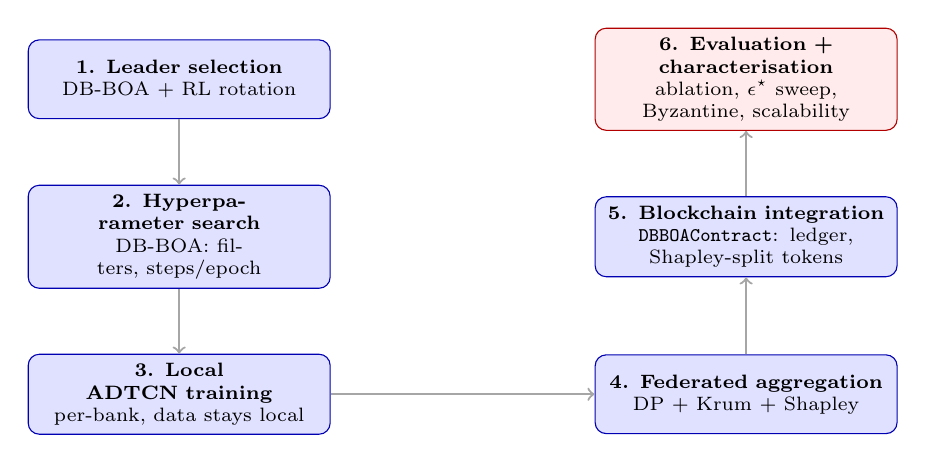
\begin{tikzpicture}[
  phase/.style={rectangle, rounded corners=4pt, draw=blue!70!black, fill=blue!12,
               minimum height=1.0cm, text width=3.6cm, align=center, font=\scriptsize},
  novel/.style={phase, draw=red!70!black, fill=red!8},
  arr/.style={->, thick, gray!70}
]
\node[phase]  (p1) at (0,0)      {\textbf{1. Leader selection}\\DB-BOA + RL rotation};
\node[phase]  (p2) at (0,-2.0)   {\textbf{2. Hyperparameter search}\\DB-BOA: filters, steps/epoch};
\node[phase]  (p3) at (0,-4.0)   {\textbf{3. Local ADTCN training}\\per-bank, data stays local};
\node[phase]  (p4) at (7.2,-4.0) {\textbf{4. Federated aggregation}\\DP + Krum + Shapley};
\node[phase]  (p5) at (7.2,-2.0) {\textbf{5. Blockchain integration}\\\texttt{DBBOAContract}: ledger, Shapley-split tokens};
\node[novel] (p6) at (7.2,0)    {\textbf{6. Evaluation + characterisation}\\ablation, $\epsilon^{\star}$ sweep, Byzantine, scalability};
\draw[arr] (p1) -- (p2);
\draw[arr] (p2) -- (p3);
\draw[arr] (p3) -- (p4);
\draw[arr] (p4) -- (p5);
\draw[arr] (p5) -- (p6);
\end{tikzpicture}
\caption{Research workflow: the six methodology phases. The highlighted final phase contains the characterisation suite around the central privacy--incentive contribution.}
\label{fig:research_workflow}
\end{figure}

\section{Summary of Contributions}
The contributions of this thesis are ordered deliberately: a primary characterisation result, a secondary suite of characterisation experiments that bounds it, and the engineering substrate that enables both. Rather than claiming algorithmic priority, this work extends prior Shapley-on-blockchain incentive systems such as FedCoin~\cite{fedcoin2020} and SI-ChainFL~\cite{zhao2026sichainfl} with a deployed Hyperledger Fabric implementation and a noise$\rightarrow$fidelity$\rightarrow$reward-error analysis.

\textbf{Primary contribution — the privacy--incentive characterisation and its fix.}
\begin{itemize}
  \item A characterisation of the privacy--incentive coupling of a Shapley-driven, chaincode-enforced reward mechanism on a real permissioned blockchain: differential privacy and contribution-based incentives are shown to be in direct tension, with the noise required for a formal privacy guarantee corrupting the contribution signal that fair on-chain rewards depend on.
  \item A concrete resolution: applying the privacy noise to the released contribution channel rather than to the shared model weights restores rank-faithful, differentially-private on-chain rewards at roughly two orders of magnitude lower privacy budget ($\epsilon^{\star}$ from $\approx 3000$ down to $\approx 50$).
\end{itemize}

\textbf{Secondary contributions — the characterisation suite that bounds the mechanism.}
\begin{itemize}
  \item The decoupling of global-model accuracy from reward fidelity under privacy noise: the two degrade at different budgets, so a model that still detects fraud can already be paying dishonest rewards.
  \item The economic isolation of a colluding majority: the Shapley-weighted reward assigns near-zero contribution weight to adversaries that out-number any statistical defence.
  \item Statistical Byzantine fault tolerance: Krum, run in the $n \ge 2f+3$ regime where its theorem holds, rejects every tested weight-poisoning attack while plain averaging collapses.
  \item The cost--fidelity limits of contribution attribution as the federation grows: exact Shapley is $O(2^n)$, and a Monte-Carlo permutation estimator keeps attribution tractable at larger federation sizes.
\end{itemize}

\textbf{Enabling substrate — the engineering on which the results rest.}
\begin{itemize}
  \item An end-to-end deployment on a real Hyperledger Fabric permissioned consortium (BankA, BankB, BankC) whose \texttt{DBBOAContract} chaincode records leader elections, consensus rounds, federation rounds, and Shapley-proportional token balances.
  \item A federated aggregation layer combining differentially private weight sharing (Gaussian mechanism), Krum robust selection, and exact / Monte-Carlo Shapley contribution attribution, bound to the on-chain token incentive.
  \item The DB-BOA hybrid metaheuristic, which automates the ADTCN detector's hyperparameter tuning and selects the consensus leader, plus a deliberately minimal linear Q-learning policy for sequential leader rotation.
\end{itemize}

\section{Scopes and Challenges}
This study focuses on financial fraud detection in a consortium banking environment, extending the DB-BOA-ADTCN framework of Prabanand and Thanabal~\cite{prabanand2025} to a Hyperledger Fabric deployment with privacy-preserving, incentive-aligned Federated Learning. The scope covers leader-node selection, model hyperparameter optimisation, differentially private and Byzantine-robust federated aggregation, Shapley-based contribution attribution, on-chain incentive enforcement, and the characterisation of the privacy--incentive coupling — all within a multi-organisation consortium evaluated primarily at three banks and stress-tested at larger sizes for the attribution layer.

Key challenges addressed include:

\begin{itemize}
\item \textbf{The privacy--incentive tension:} Differential privacy noise, added to protect shared parameters, corrupts the contribution signal that fair rewards depend on; the framework must locate the operating regime and channel placement in which rewards remain faithful under a formal privacy guarantee.
\item \textbf{Computational overhead:} DB-BOA's population-based search is applied across distinct optimisation tasks per training run. Population sizes and iteration counts were tuned (population: 15--20, iterations: 20--30) to maintain practical runtimes while preserving solution quality.
\item \textbf{Data heterogeneity:} The banks hold different proportions of training data (50/30/20 split), creating non-IID conditions that stratified partitioning and the contribution-weighted aggregation must accommodate.
\item \textbf{Adversarial participation:} Both weight-level poisoning (countered by Krum in its $n\ge 2f+3$ regime) and behavioural collusion (countered by economic isolation through the Shapley-weighted reward) are simulated to test the complementary statistical and economic defences.
\item \textbf{Blockchain determinism:} Hyperledger Fabric requires all chaincode logic to be fully deterministic. All DB-BOA optimisation and randomness was confined to the off-chain Python layer; only finalised results (leader ID, token deltas, contribution weights, model accuracy) were written to the ledger.
\item \textbf{Scalability of contribution attribution:} Exact Shapley is $O(2^n)$ and becomes infeasible beyond roughly a dozen organisations; a Monte-Carlo permutation estimator keeps contribution attribution tractable to larger federations. The scalability claim is therefore for \emph{contribution attribution}, not for blockchain throughput or distributed training, which remain outside scope.
\end{itemize}

Differential privacy (Gaussian mechanism) is already integrated into the weight-sharing and incentive layers; future directions include relaxing the privacy budget with DP-SGD, extending the consortium beyond three organisations in a live deployment, deploying across real multi-host banking nodes, and investigating quantum-resistant cryptographic primitives for long-term ledger integrity.
